\scanpage{83}
\mspage{82}
is equipped with an element \inserted{$\handwritten{\underline}{f}_q$} of $G_{\deleted{a}\handwritten{\nu}}(K_{\deleted{a}\handwritten{\nu}})$\inserted{(\handwritten{``}Frobenius relative to $\handwritten{\underline}{F}_q$'')}\handwritten{\begin{tikzpicture}[baseline=0cm,x=1cm,y=1cm]\draw[thin] (0,-.15)..controls (-.08,.1) and (.1,.18)..(.23,.18)--(3.5,.18)..controls (3.6,.17) and (3.7,.28)..(3.66,.38);\end{tikzpicture}}. The latter is moreover none other than $\deleted{\handwritten{\underline}{f}_q}$ $\handwritten{\underline}{f}^{\deleted{a}\handwritten{\nu}}$, where $\handwritten{\underline}{f}$ is the canonical generator of $G$ (the \unsure{\rlap{l}a|\rlap{d}a}bsolute Frobenius \handwritten{!}). \deleted{\unsure{O|C} one therefore sees that $G_a$ is again generated by} Note that $a\operatorname{\rlap{i}Id}_G$ is a monomorphis\rlap{e}m\unsure{\rlap{d}|\rlap{r}|} (for $x\handwritten{\mathrel{\begin{tikzpicture}[baseline=-.04cm,x=1cm,y=1cm]\draw[semithick] (0,-.1)--(0,.12) (0,0)--(.55,0) (.55,-.06)--(.55,.06);\end{tikzpicture}}}x^{\deleted{a}\handwritten{\nu}}$ is an epimorphism in $\handwritten{\overline}{\handwritten{\underline}{Q}}_{\handwritten{p}}^{\handwritten{*}}$ ), hence \rlap{x}induces an isomorphism between $\rlap{$K$}G_{K_{\deleted{a}\handwritten{\nu}}}$ and $G_{\deleted{a}\handwritten{\nu}}\handwritten{\simeq}G(\handwritten{\underline}{F}_q)$,trans\rlap{o}f\rlap{f}orming the \deleted{relati} absolute frobenius into the frobenius relative to $\handwritten{\underline}{F}_q$. Thanks to this, one sees:

\handwritten{\uline}{Proposition} 10.1. The \inserted{Tannakian}\handwritten{\begin{tikzpicture}[baseline=0cm,x=1cm,y=1cm]\draw[thin] (0,-.15)..controls (-.08,.1) and (.1,.18)..(.23,.18)--(0.8,.18)..controls (0.9,.17) and (1.0,.28)..(0.9600000000000001,.38);\end{tikzpicture}} category $\operatorname{Fcriso}(\handwritten{\underline}{F}_q)\handwritten{\otimes}_{\overset{\mathrm{Fr.}}{\handwritten{\underline}{Q}}_p}K_a$ is equivalent to the \inserted{Tannakian}\handwritten{\begin{tikzpicture}[baseline=0cm,x=1cm,y=1cm]\draw[thin] (0,-.15)..controls (-.08,.1) and (.1,.18)..(.23,.18)--(0.8,.18)..controls (0.9,.17) and (1.0,.28)..(0.9600000000000001,.38);\end{tikzpicture}} category $\operatorname{Fcriso}(\handwritten{\underline}{F}_p)\handwritten{\otimes}_{\handwritten{\underline}{Q}_p}K_a$,\handwritten{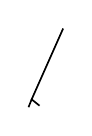
\begin{tikzpicture}[baseline=-.02cm,x=1cm,y=1cm]\draw[semithick] (.4,.9)--(0,0)--(.1,-.08);\draw[semithick] (0,0)--(-.04,-.1);\end{tikzpicture}} \margin{\handwritten{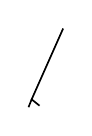
\begin{tikzpicture}[baseline=-.02cm,x=1cm,y=1cm]\draw[semithick] (.4,.9)--(0,0)--(.1,-.08);\draw[semithick] (0,0)--(-.04,-.1);\end{tikzpicture}}\handwritten{i.e. the category of pairs $(E,F'_E)$ of a vector space over $K_\nu$ and an automorphism of this vector space....)}}
with $\handwritten{\underline}{f}_q$ corresponding to $\handwritten{\underline}{f}^{\deleted{a}\handwritten{\nu}}$ (where one can, if one wishes, consider $\handwritten{\underline}{f}_q$ and $\handwritten{\underline}{f}$ as end\rlap{m}o\unsure{\rlap{E}m|\rlap{h}m|m}orphisms of the identity functors of $\operatorname{Fcriso}(\handwritten{\underline}{F}_q)$ resp. $\operatorname{Fcriso}(\handwritten{\underline}{F}_p)$)), and corres\deleted{p}pondence of the canonical fiber functors. The functor deduced from the ch\rlap{n}a\rlap{a}nge of base $\handwritten{\underline}{F}_p\handwritten{\to}\handwritten{\underline}{F}_q$

\[
\operatorname{Fcriso}(\handwritten{\underline}{F}_{\unsure{\rlap{g}p|\rlap{q}p|p}})\handwritten{\otimes}_{\overset{\mathrm{Fr.}}{\handwritten{\underline}{Q}}_p}K_{\deleted{a}\handwritten{\nu}}\handwritten{\longrightarrow}\operatorname{Fcriso}(\handwritten{\underline}{F}_q)\handwritten{\otimes}_{\handwritten{\underline}{Q}_p}K_{\deleted{a}\handwritten{\nu}}
\]
\unsure{\rlap{n}is|\rlap{e}is|is} identified, by the preceding equivalence, with the functor which to any pair $(E,F_E)$ of a vector space over $K_{\deleted{a}\handwritten{\nu}}$ and an automorphism thereof, associates the pair $(E,F_E{}^{\deleted{a}\handwritten{\nu}})$\handwritten{;}
\inserted{\handwritten{analogous \unsure{fo\textsuperscript{r}|for} $\operatorname{Fcriso}(F_1)-\operatorname{Fcriso}(F_q)\otimes_{\mathbb{Q}_p}K_\nu$, it is identified: $(E,F_E)\longmapsto(E,F_E{}^\nu)$.}}

10.2. Since one knows $\handwritten{\underline}{G}(\handwritten{\underline}{F}_q)$ as a subgerbe $\handwritten{\underline}{G}_{\deleted{a}\handwritten{\nu}}$ of $\handwritten{\underline}{G}=\handwritten{\underline}{G}(\handwritten{\underline}{F}_p)$, and since this contains $\handwritten{\underline}{H}$, one therefore knows in principle \rlap{d}the inclusion
\[
\handwritten{\underline}{H}\handwritten{\longrightarrow}\handwritten{\underline}{G}_{\deleted{a}\handwritten{\nu}}=\handwritten{\underline}{G}(F_q)\quad ,
\]
hence also the functor
\[
\operatorname{Rep}(\handwritten{\underline}{G}_{\deleted{a}\handwritten{\nu}})\handwritten{\simeq}\operatorname{Fcriso}(\handwritten{\underline}{F}_q)\handwritten{\mathrel{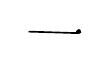
\begin{tikzpicture}[baseline=-.04cm,x=1cm,y=1cm]\draw[semithick] (0,0)--(.65,-.02);\fill (.59,-.02)..controls (.62,.05) and (.67,.05)..(.67,-.02)--cycle;\end{tikzpicture}}}\operatorname{Rep}(\handwritten{\underline}{H})\quad ,
\]
\deleted{\inserted{and} Consider the corresponding functor}
\[
\deleted{\operatorname{\unsure{\rlap{R}F|\rlap{K}F|F}criso}(\handwritten{\underline}{F}_q)\handwritten{\otimes}_{\handwritten{\underline}{Q}_p}K_{\underset{\deleted{a}}{a}}\quad\operatorname{Rep}(\handwritten{\underline}{H})\handwritten{\otimes}_{\handwritten{\underline}{Q}_p}K_a\ .}
\]
\figure{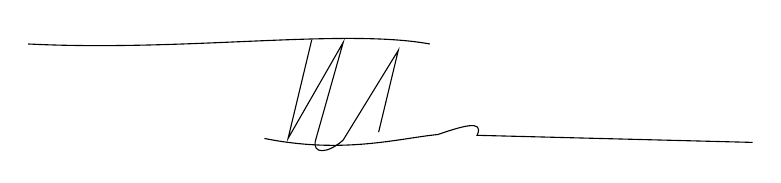
\begin{tikzpicture}[x=1cm,y=1cm]\draw[thin] (0,1.3)..controls (2,1.2) and (4,1.5)..(5.1,1.3);\draw[thin] (3.6,1.35)--(3.3,.1)--(4,1.32)--(3.65,.08)..controls (3.6,-.1) and (3.8,-.1)..(4,.08)--(4.7,1.22)--(4.45,.18);\draw[thin] (3,.1)..controls (4,-.1) and (4.7,.1)..(5.2,.15)..controls (5.5,.25) and (5.8,.35)..(5.7,.14)--(9.2,.05);\end{tikzpicture}}
The effect of this\deleted{s} functor\deleted{s} on the isomorphism classes of elements is known (as whenever one is dealing with a morphism from a \deleted{gerbe of} Tannakian \unsure{\rlap{O}c|\rlap{C}c}ategory with commutative band to another with band of multiplicative type) through knowl\rlap{n}e\rlap{a}dge of the corresponding homomorphism of bands
